\documentclass{article}%
\usepackage[T1]{fontenc}%
\usepackage[utf8]{inputenc}%
\usepackage{lmodern}%
\usepackage{textcomp}%
\usepackage{lastpage}%
\usepackage{geometry}%
\geometry{margin=0.5in,headheight=10pt,footskip=0.2in,tmargin=0.5in,bmargin=0.5in}%
\usepackage{graphicx}%
\usepackage{float}%
\usepackage{booktabs}%
\usepackage{hyperref}%
\usepackage{caption}%
\usepackage{subcaption}%
\usepackage{ragged2e}%
%
\title{ML Raport}%
\author{AutoPrep}%
\date{\today}%
%
\begin{document}%
\normalsize%
\maketitle%

    \begin{abstract}
    This raport has been generated with AutoPrep.
    \end{abstract}
    %
\tableofcontents%
\newpage%
\section{Overview}%
\label{sec:Overview}%

%
\subsection{System}%
\label{subsec:System}%

%


\begin{table}[H]%
\begin{center}%
\begin{tabular}{l l}%
\hline%
System&Windows\\%
Machine&AMD64\\%
Processor&Intel64 Family 6 Model 140 Stepping 2, GenuineIntel\\%
Architecture&64bit\\%
Python Version&3.11.5\\%
Physical Cores&4\\%
Logical Cores&8\\%
CPU Frequency (MHz)&1207.00\\%
Total RAM (GB)&15.74\\%
Available RAM (GB)&1.66\\%
Total Disk Space (GB)&457.28\\%
Free Disk Space (GB)&234.67\\%
\hline%
\end{tabular}%
\end{center}%
\caption{System overview.}%
\end{table}

%
\subsection{Dataset}%
\label{subsec:Dataset}%

%


\begin{table}[H]%
\begin{center}%
\begin{tabular}{l l}%
\hline%
Number of samples&1047\\%
Number of features&13\\%
Number of numerical features&6\\%
Number of categorical features&7\\%
\hline%
\end{tabular}%
\end{center}%
\caption{Dataset Summary.}%
\end{table}

%


\begin{table}[H]%
\begin{center}%
\begin{tabular}{l l l}%
\hline%
\textbf{class}&\textbf{number of observations}&\textbf{Percentage}\\%
\hline%
0&665&0.64\\%
1&382&0.36\\%
\hline%
\end{tabular}%
\end{center}%
\caption{Target class distribution.}%
\end{table}

%


\begin{table}[H]%
\begin{center}%
\begin{tabular}{l l l}%
\hline%
\textbf{classgit}&\textbf{number of observations}&\textbf{Percentage}\\%
\hline%
pclass&0&0.00\\%
name&0&0.00\\%
sex&0&0.00\\%
age&207&0.20\\%
sibsp&0&0.00\\%
parch&0&0.00\\%
ticket&0&0.00\\%
fare&1&0.00\\%
cabin&813&0.78\\%
embarked&1&0.00\\%
boat&672&0.64\\%
body&948&0.91\\%
home\_\_dest&453&0.43\\%
\hline%
\end{tabular}%
\end{center}%
\caption{Missing values distribution.}%
\end{table}

%


\begin{table}[H]%
\begin{center}%
\begin{tabular}{l l l l}%
\hline%
\textbf{class}&\textbf{type}&\textbf{dtype}&\textbf{space usage}\\%
\hline%
pclass&numerical&int64&16.8 kB\\%
name&categorical&object&96.4 kB\\%
sex&categorical&category&9.7 kB\\%
age&numerical&float64&16.8 kB\\%
sibsp&numerical&int64&16.8 kB\\%
parch&numerical&int64&16.8 kB\\%
ticket&categorical&object&75.1 kB\\%
fare&numerical&float64&16.8 kB\\%
cabin&categorical&object&48.6 kB\\%
embarked&categorical&category&9.7 kB\\%
boat&categorical&object&51.8 kB\\%
body&numerical&float64&16.8 kB\\%
home\_\_dest&categorical&object&68.2 kB\\%
\hline%
\end{tabular}%
\end{center}%
\caption{Features dtypes description.}%
\end{table}

%


\begin{table}[H]%
\begin{center}%
\begin{tabular}{l l l l l l l l l}%
\hline%
\textbf{index}&\textbf{count}&\textbf{mean}&\textbf{std}&\textbf{min}&\textbf{25\%}&\textbf{50\%}&\textbf{75\%}&\textbf{max}\\%
\hline%
pclass&1047.00&2.30&0.84&1.00&2.00&3.00&3.00&3.00\\%
age&840.00&29.53&14.27&0.17&21.00&28.00&38.62&80.00\\%
sibsp&1047.00&0.52&1.05&0.00&0.00&0.00&1.00&8.00\\%
parch&1047.00&0.40&0.89&0.00&0.00&0.00&0.00&9.00\\%
fare&1046.00&33.55&51.81&0.00&7.92&14.50&31.27&512.33\\%
body&99.00&160.90&98.35&1.00&73.50&156.00&255.50&328.00\\%
\hline%
\end{tabular}%
\end{center}%
\caption{Numerical features description.}%
\end{table}

%


\begin{table}[H]%
\begin{center}%
\begin{tabular}{l l l l l}%
\hline%
\textbf{index}&\textbf{count}&\textbf{unique}&\textbf{top}&\textbf{freq}\\%
\hline%
name&1047&1046&Connolly, Miss. Kate&2\\%
ticket&1047&773&CA. 2343&9\\%
cabin&234&161&B57 B59 B63 B66&5\\%
boat&375&25&13&34\\%
home\_\_dest&594&317&New York, NY&50\\%
\hline%
\end{tabular}%
\end{center}%
\caption{Categorical features description.}%
\end{table}

%
\section{Eda}%
\label{sec:Eda}%

%
This part of the report provides basic insides to the data and the informations it holds..%
\subsection{Eda}%
\label{subsec:Eda}%

%


\begin{figure}[H]%
\centering%
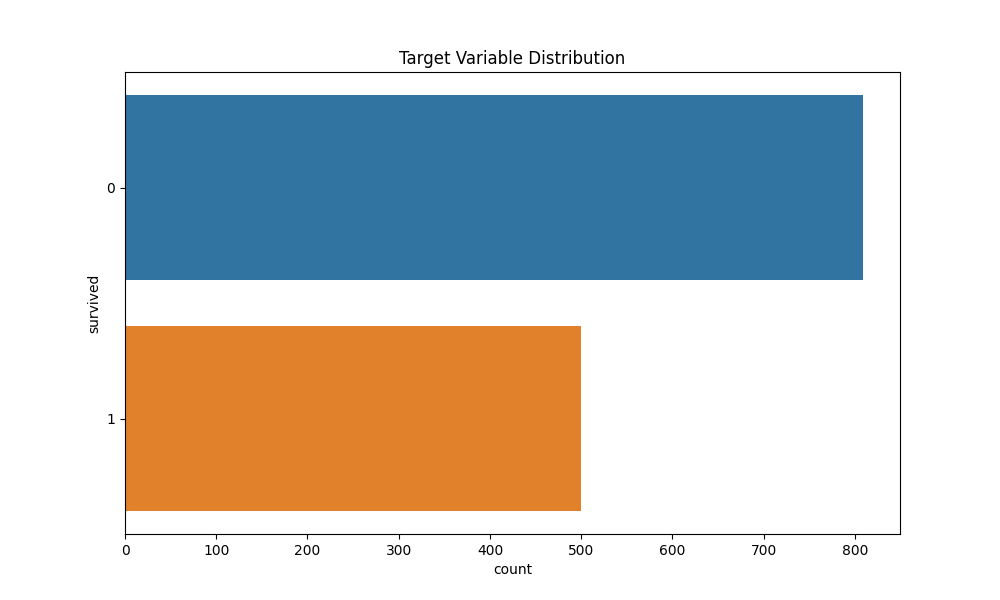
\includegraphics[width=0.9\textwidth]{C:/Users/rogal/MojGithub/AutoPrep/examples/raport/raport/charts/target_distribution.png}%
\caption{Target distribution.}%
\end{figure}

%


\begin{figure}[H]%
\centering%
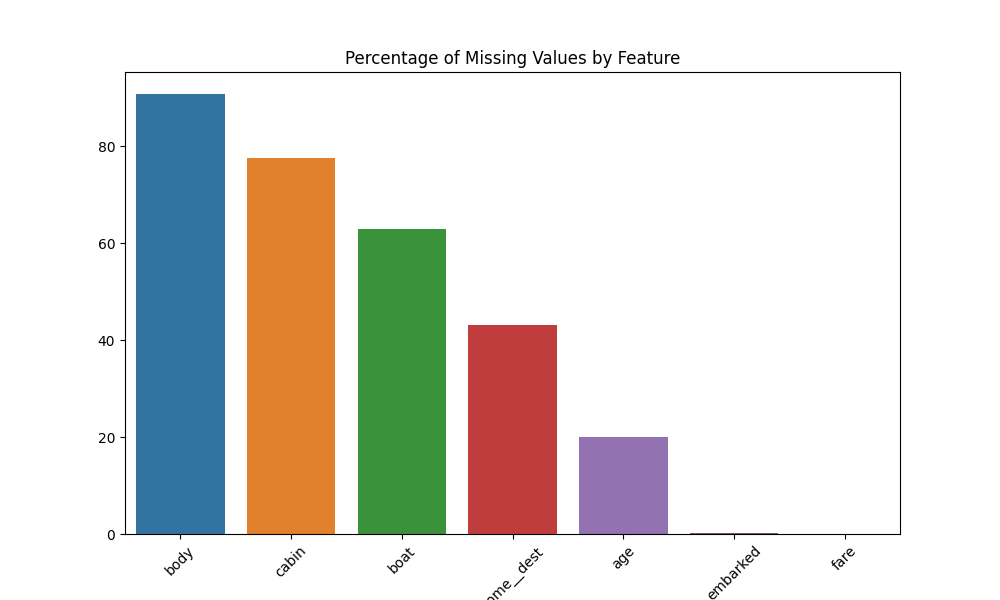
\includegraphics[width=0.9\textwidth]{C:/Users/rogal/MojGithub/AutoPrep/examples/raport/raport/charts/missing_values.png}%
\caption{Missing values.}%
\end{figure}

%
\subsection{Categorical}%
\label{subsec:Categorical}%

%


\begin{figure}[H]%
\centering%
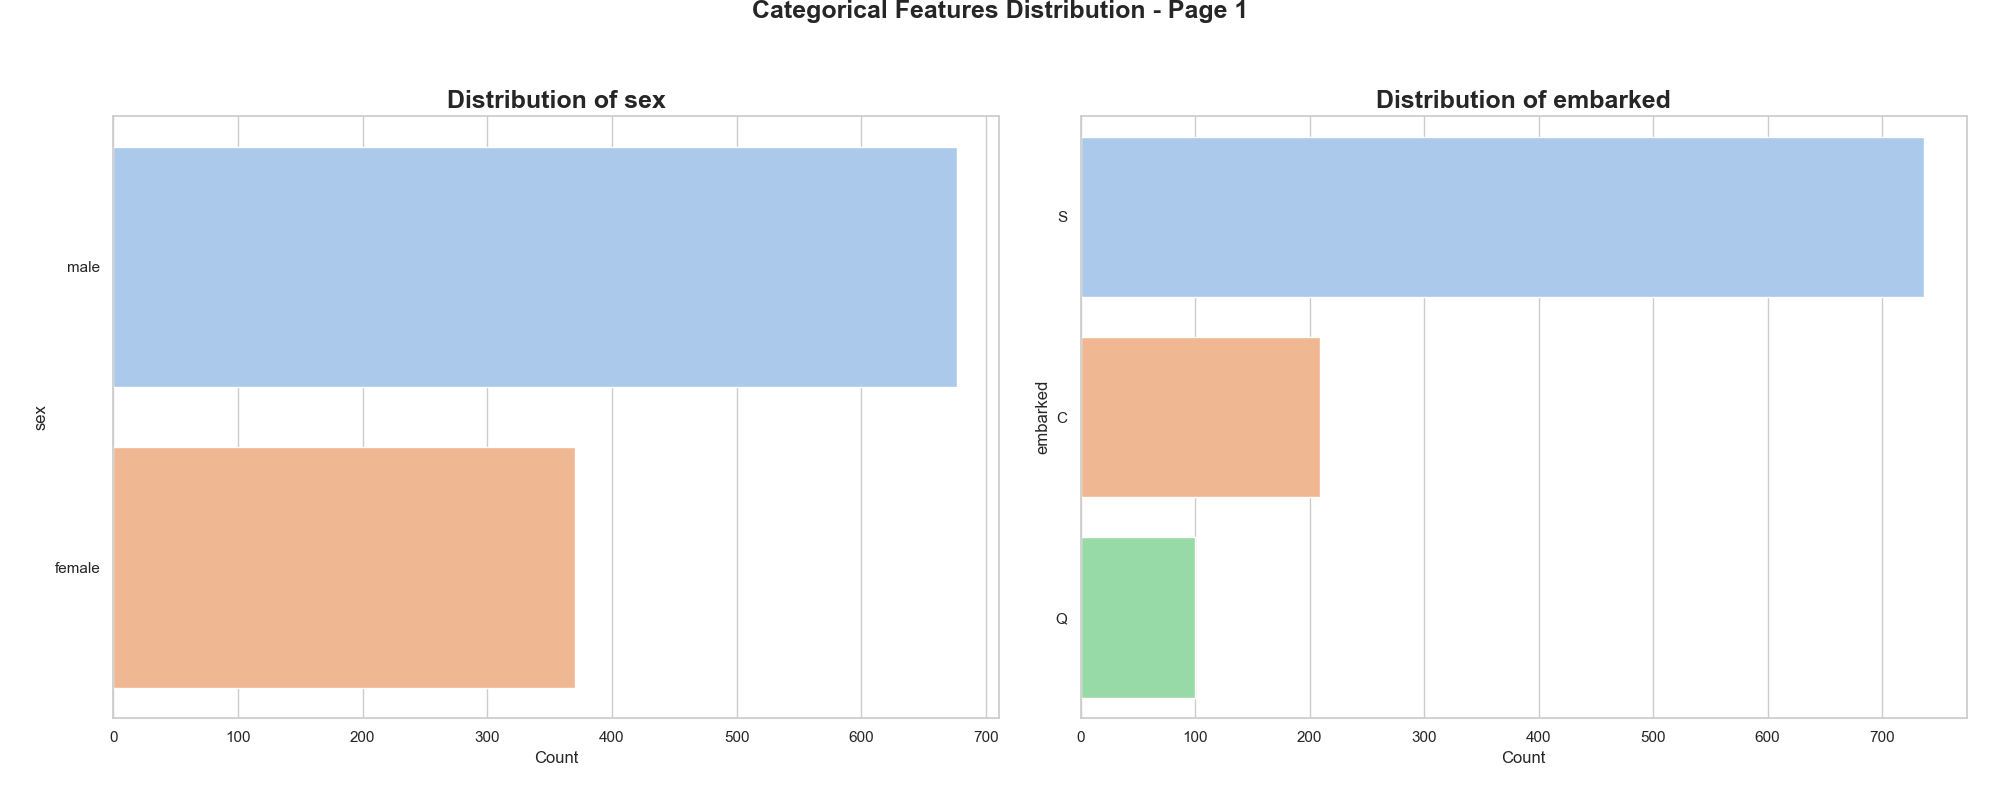
\includegraphics[width=0.9\textwidth]{C:/Users/rogal/MojGithub/AutoPrep/examples/raport/raport/charts/categorical_distribution_page_1.png}%
\caption{Categorical Features Distribution {-} Page 1}%
\end{figure}

%
\subsection{Numerical}%
\label{subsec:Numerical}%

%


\begin{figure}[H]%
\centering%
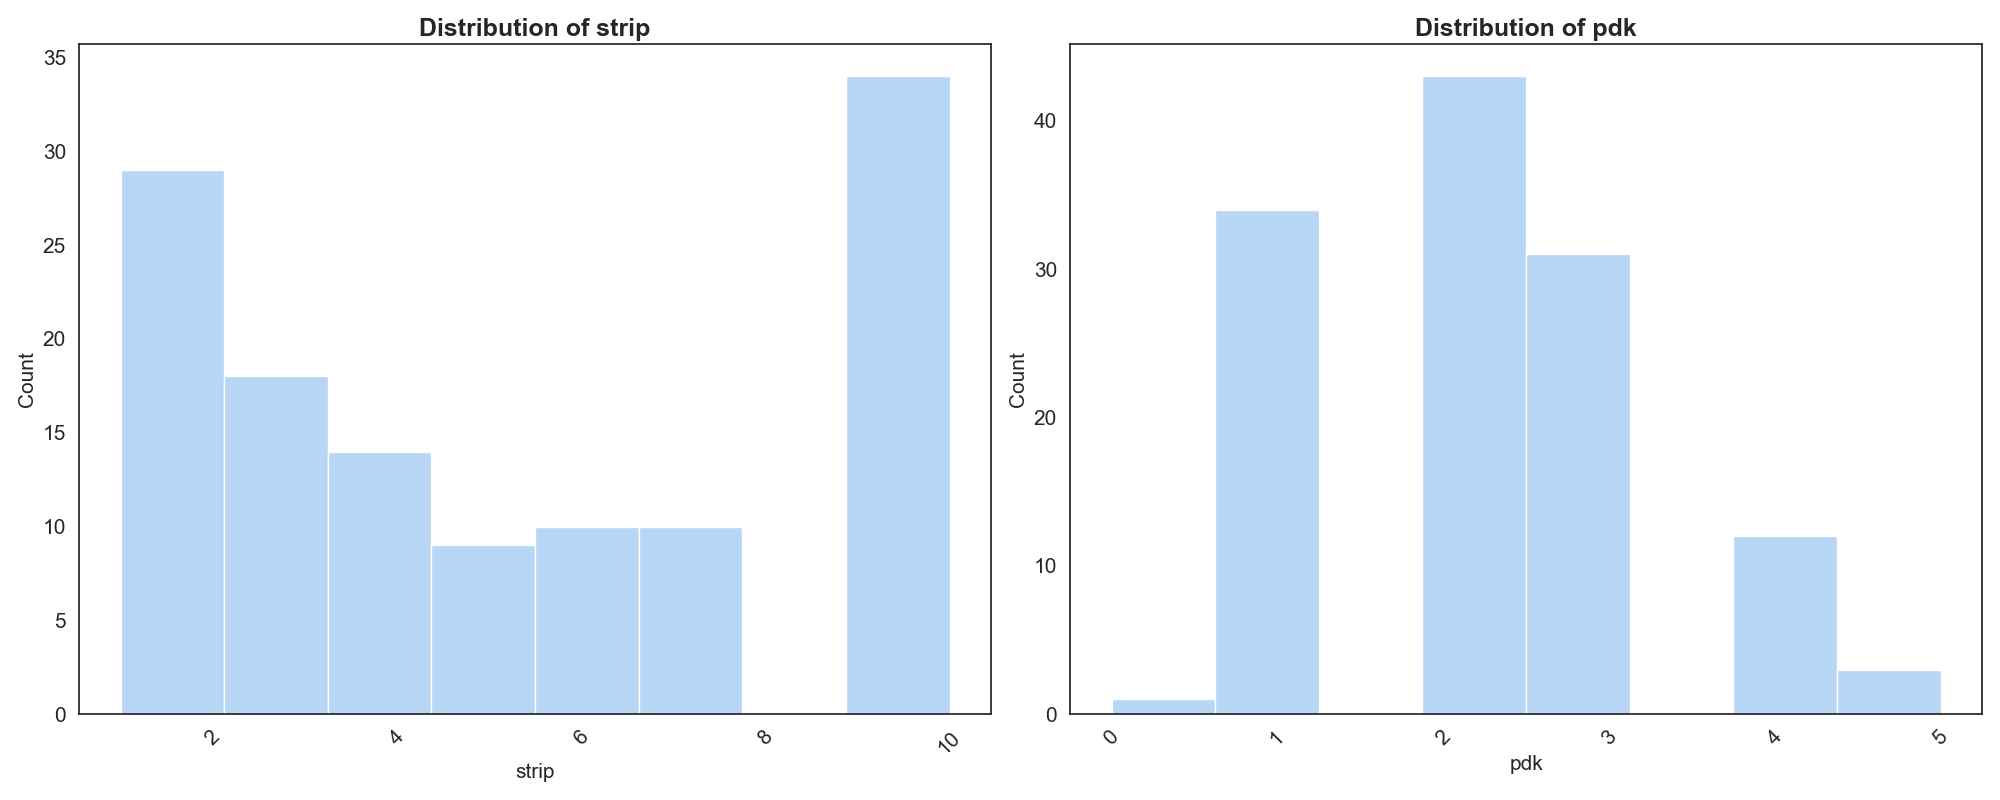
\includegraphics[width=0.9\textwidth]{C:/Users/rogal/MojGithub/AutoPrep/examples/raport/raport/charts/numerical_distribution_page_1.png}%
\caption{Numerical Features Distribution {-} Page 1}%
\end{figure}

%


\begin{figure}[H]%
\centering%
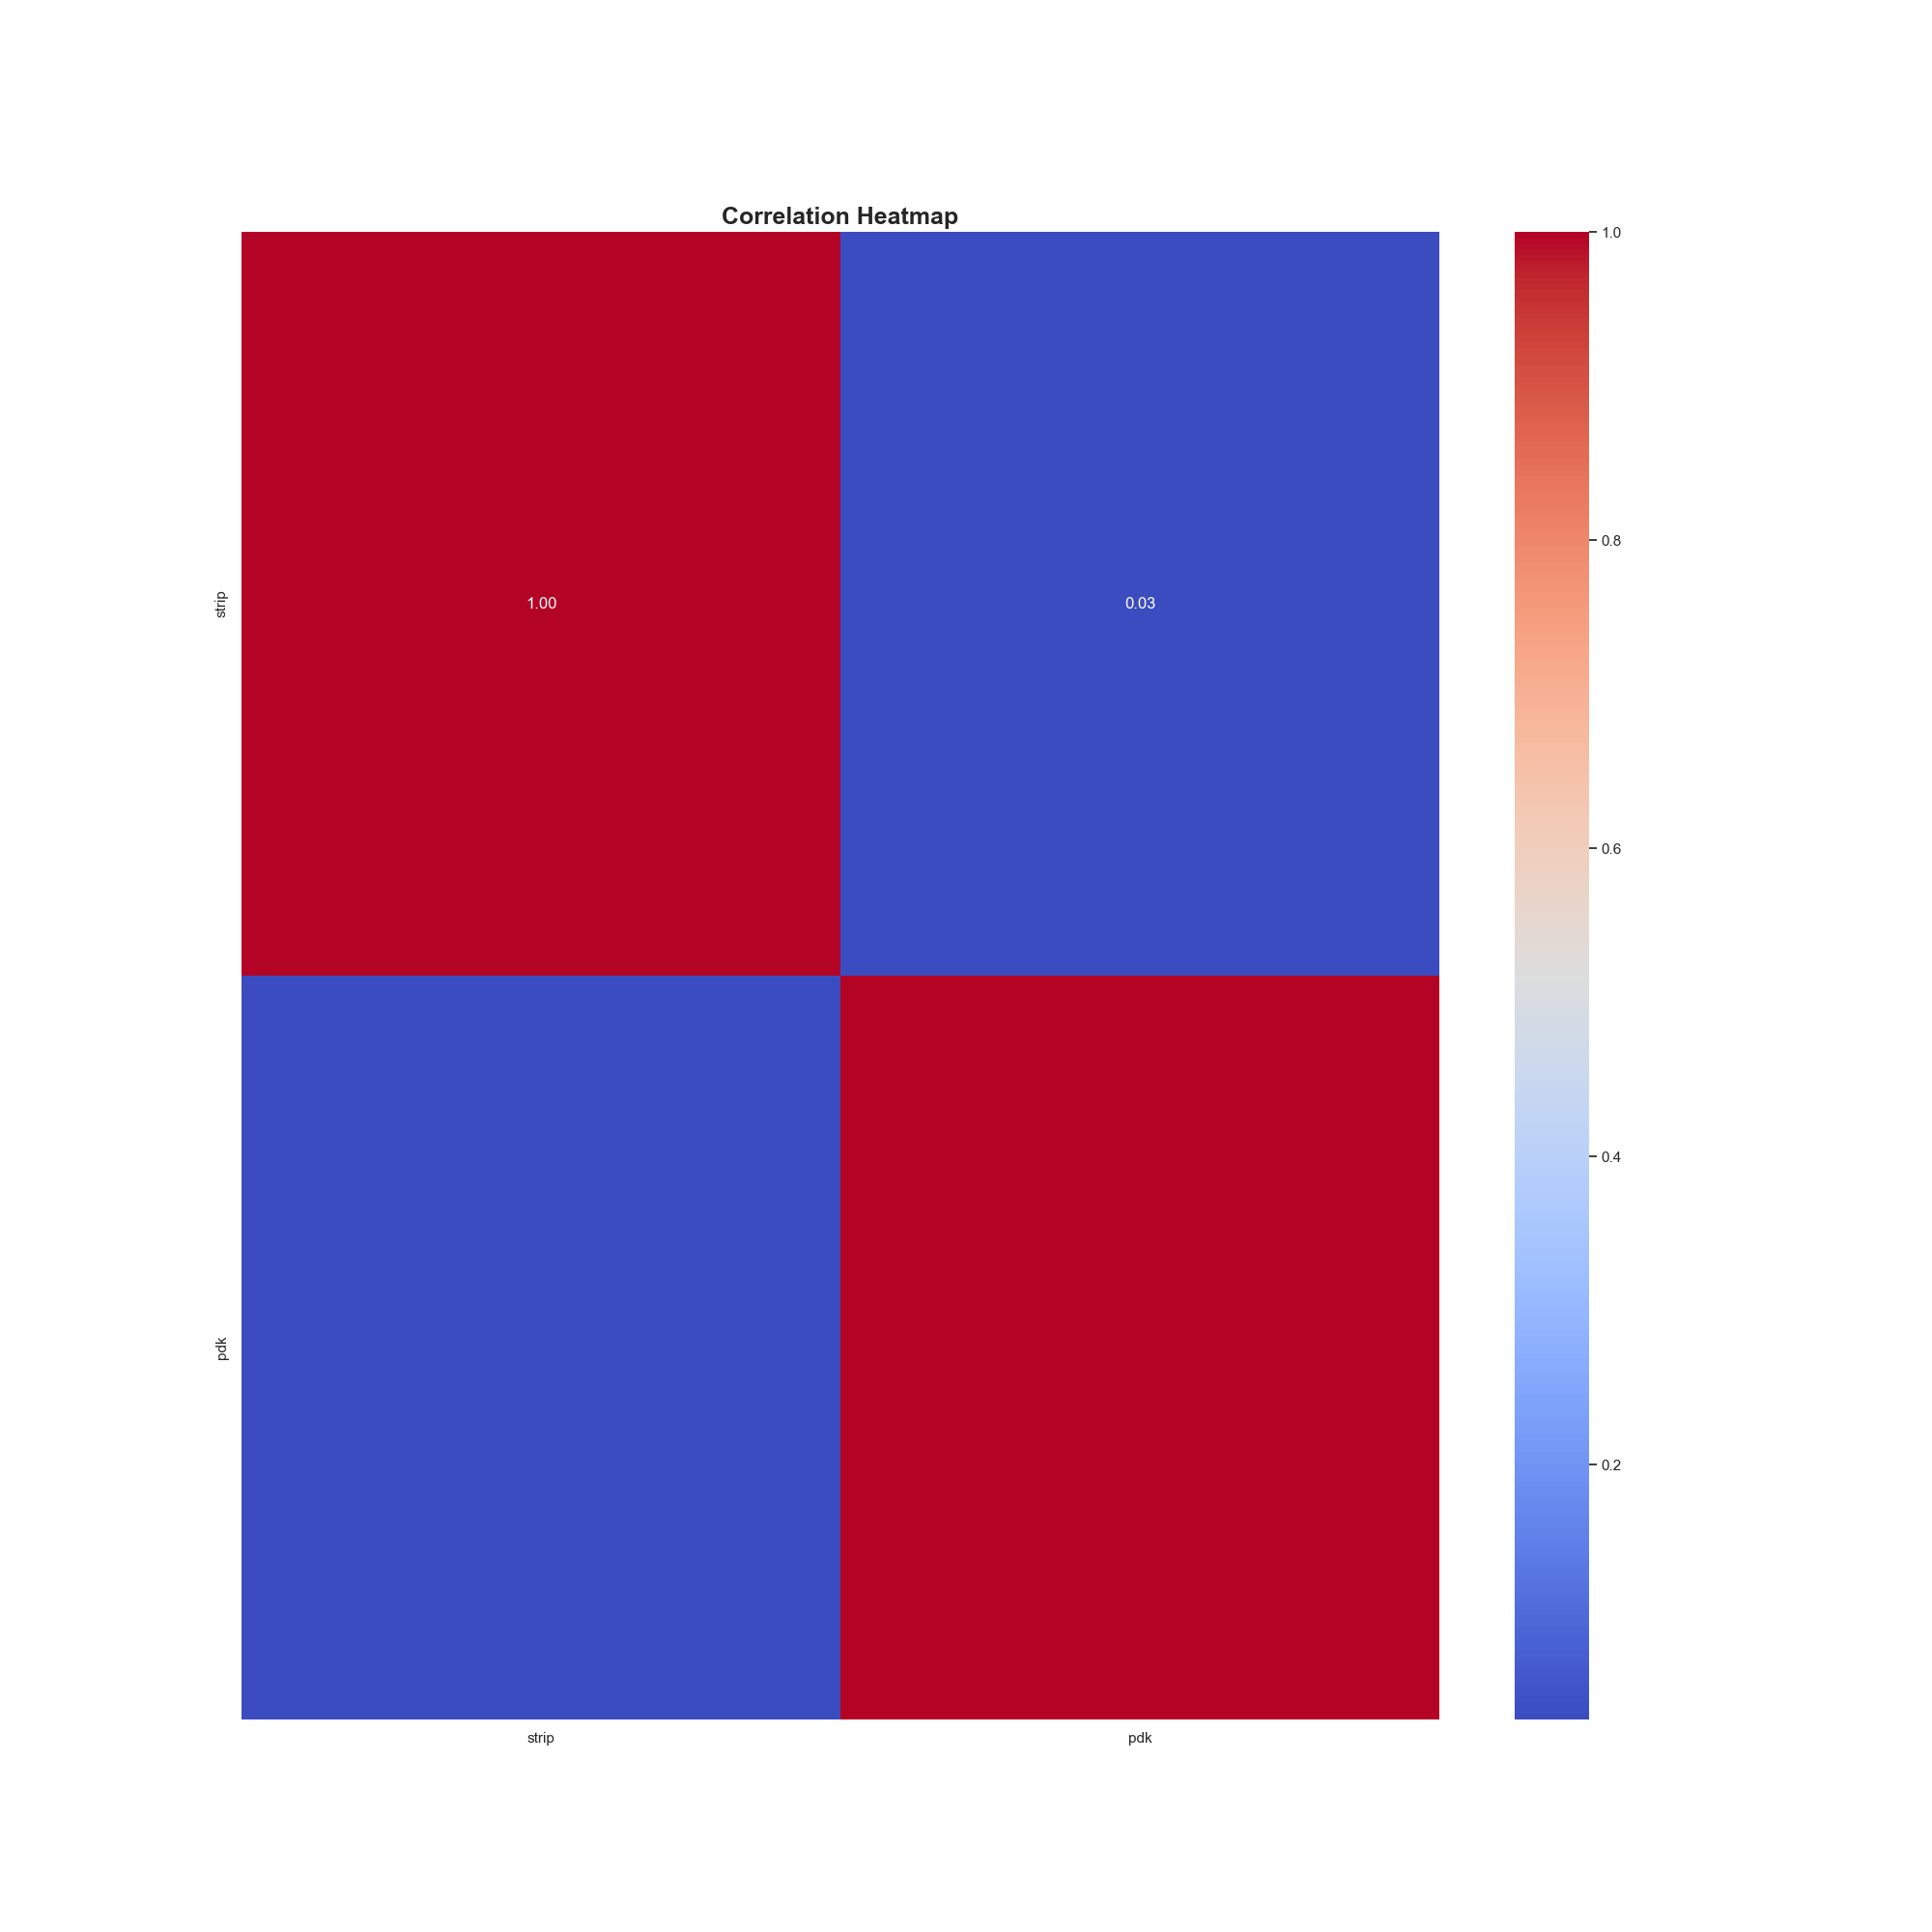
\includegraphics[width=0.9\textwidth]{C:/Users/rogal/MojGithub/AutoPrep/examples/raport/raport/charts/correlation_heatmap.png}%
\caption{Correlation heatmap.}%
\end{figure}

%


\begin{figure}[H]%
\centering%
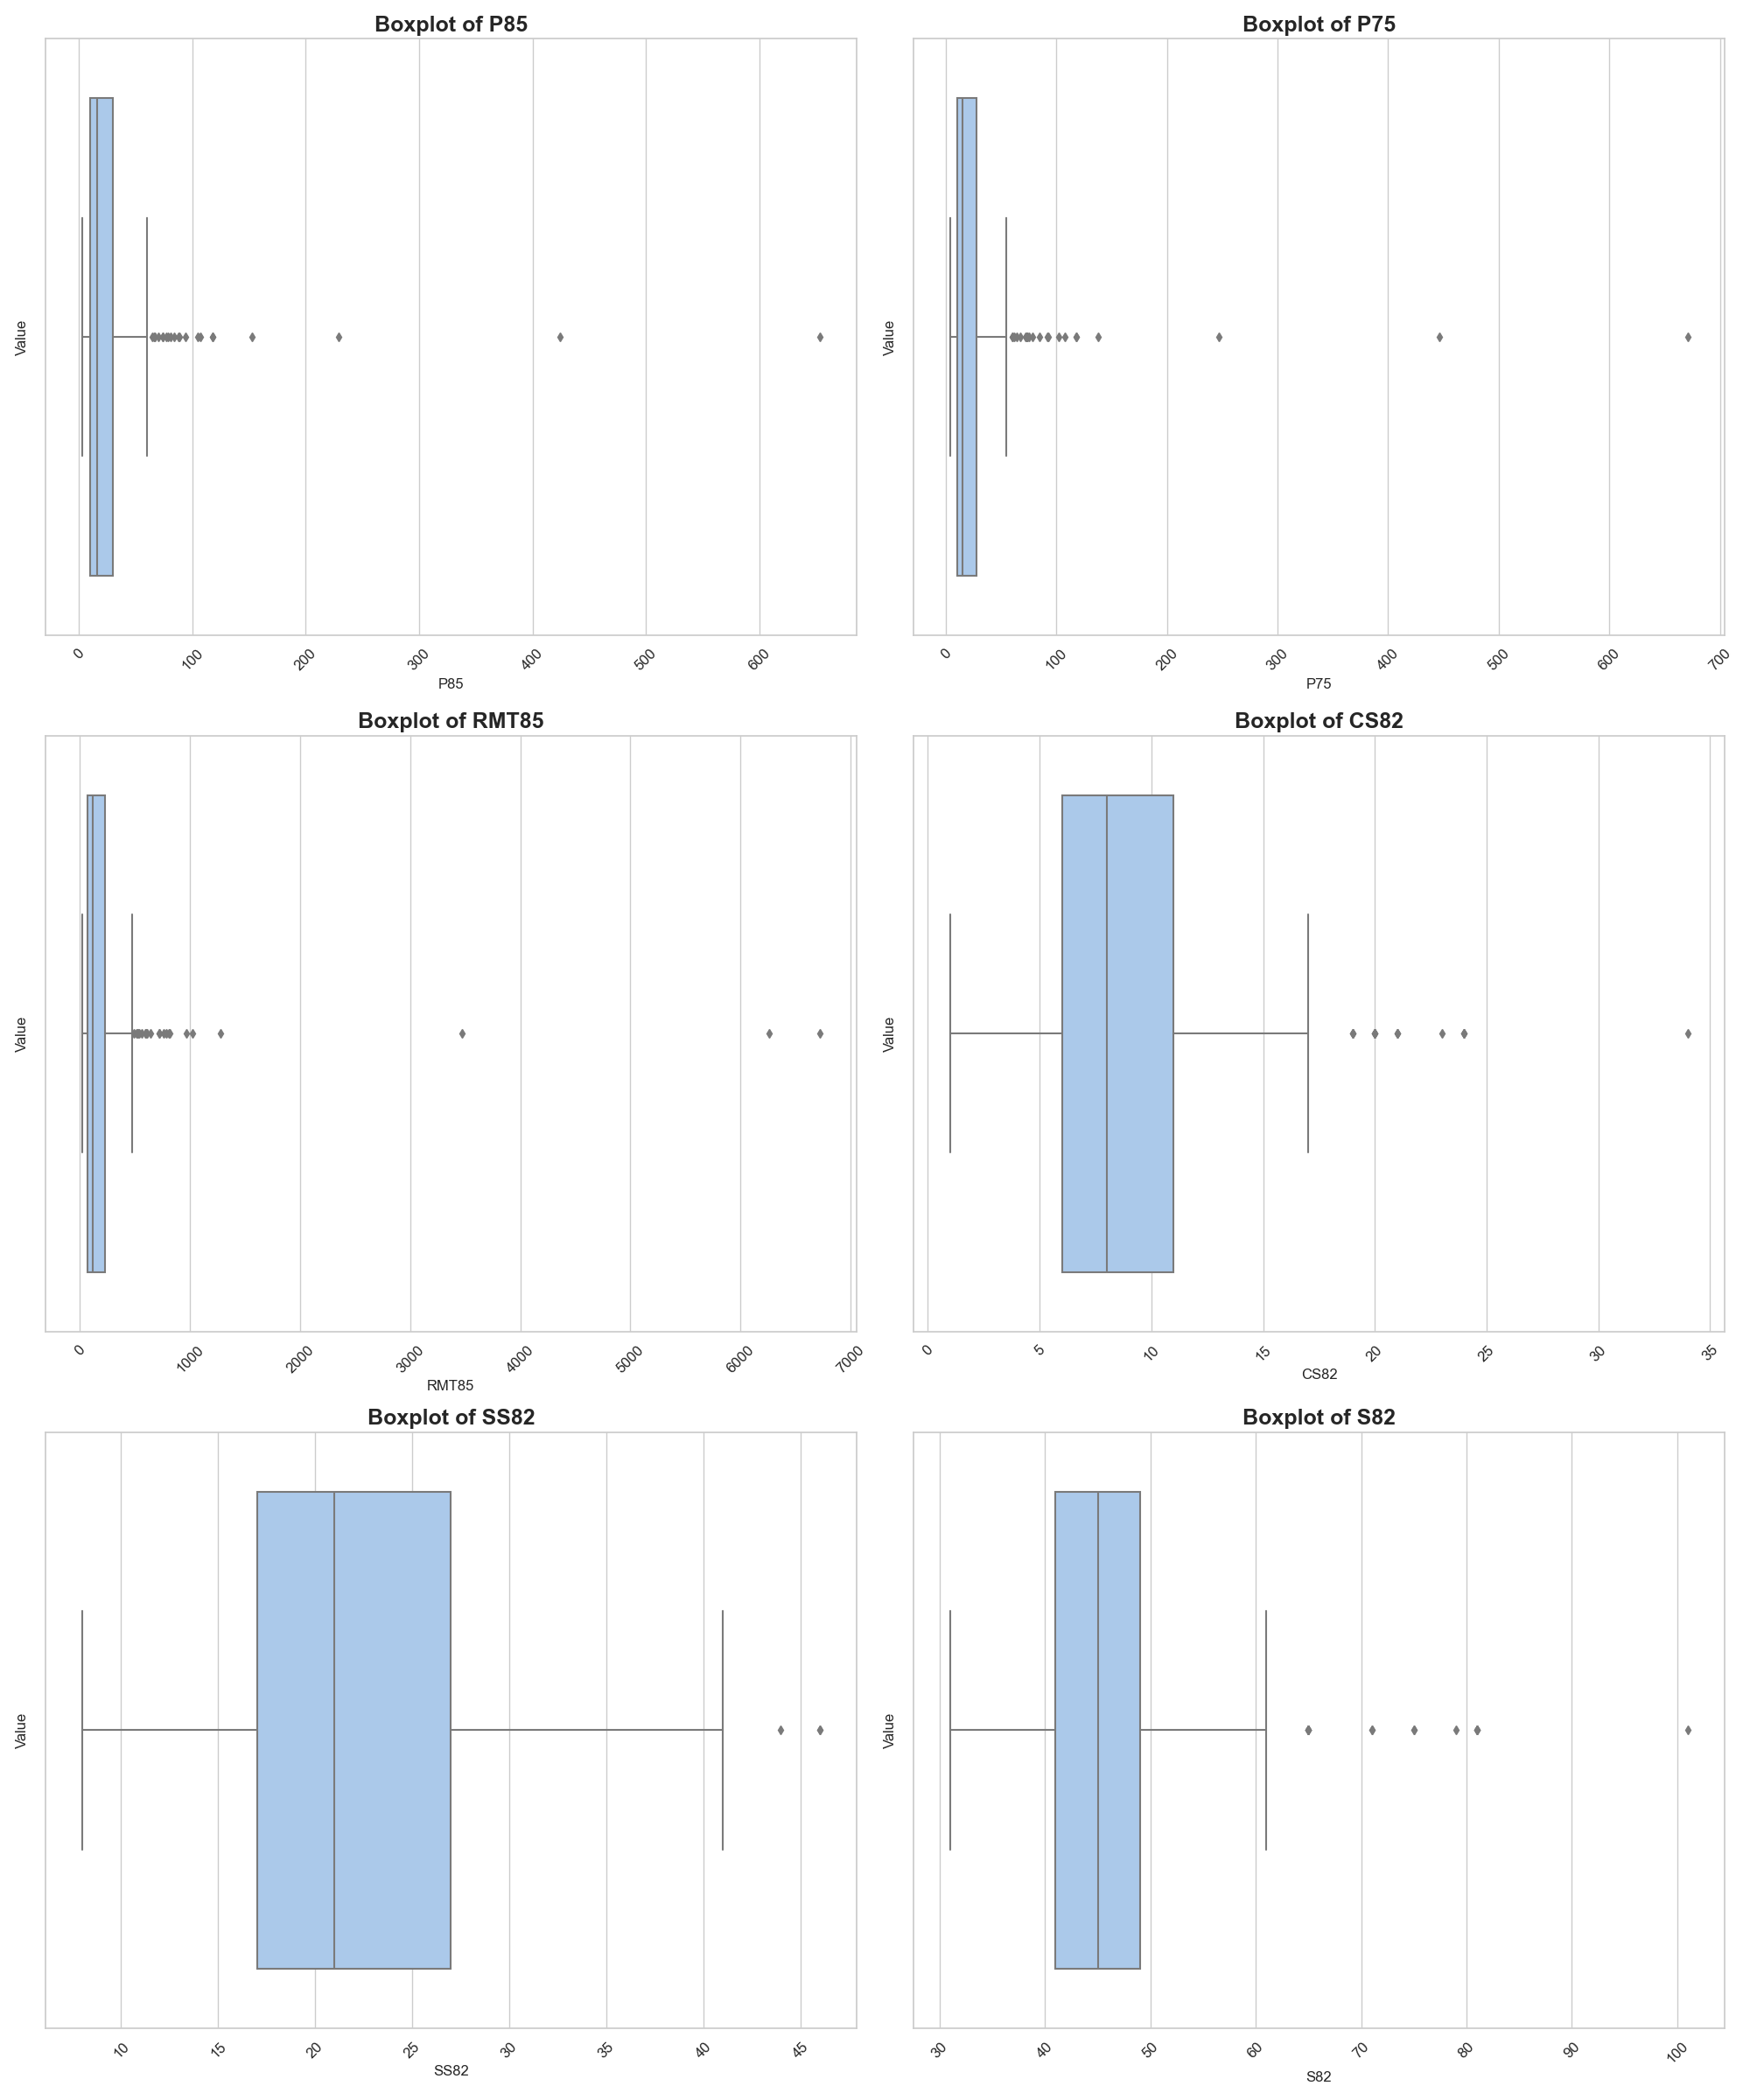
\includegraphics[width=0.9\textwidth]{C:/Users/rogal/MojGithub/AutoPrep/examples/raport/raport/charts/boxplot_page_1.png}%
\caption{Boxplot page 1}%
\end{figure}

%
\section{Preprocessing}%
\label{sec:Preprocessing}%

%
This part of the report presents the results of the preprocessing process. It was configured to create up to 3 unique preprocessing pipelines.%


\begin{table}[H]%
\begin{center}%
\begin{tabular}{l l}%
\hline%
\textbf{Category}&\textbf{Value}\\%
\hline%
Unique created pipelines&1\\%
All created pipelines (after exploading each step params)&3\\%
All pipelines fit time&3 seconds\\%
All pipelines score time&3 seconds\\%
scores\_count&3.00\\%
scores\_mean&0.75\\%
scores\_std&0.00\\%
scores\_min&0.75\\%
scores\_25\%&0.75\\%
scores\_50\%&0.75\\%
scores\_75\%&0.75\\%
scores\_max&0.75\\%
Scoring function&<class 'str'>\\%
Scoring model&RandomForestClassifier\\%
\hline%
\end{tabular}%
\end{center}%
\caption{Preprocessing pipelines runtime statistics.}%
\end{table}

%


\begin{table}[H]%
\begin{center}%
\begin{tabular}{p{20mm} p{160mm}}%
\hline%
\textbf{index}&\textbf{steps}\\%
\hline%
0&NAImputer, UniqueFilter, ColumnEncoder, VarianceFilter, CorrelationFilter, ColumnScaler\\%
\hline%
\end{tabular}%
\end{center}%
\caption{Pipelines steps overview.}%
\end{table}

%


\begin{table}[H]%
\begin{center}%
\begin{tabular}{l l l l l}%
\hline%
\textbf{score index}&\textbf{file name}&\textbf{score}&\textbf{fit duration}&\textbf{score duration}\\%
\hline%
0&preprocessing\_pipeline\_0.joblib&0.75&a moment&a moment\\%
1&preprocessing\_pipeline\_1.joblib&0.75&a moment&a moment\\%
2&preprocessing\_pipeline\_2.joblib&0.75&a moment&a moment\\%
\hline%
\end{tabular}%
\end{center}%
\caption{Best preprocessing pipelines.}%
\end{table}

%


\begin{table}[H]%
\begin{center}%
\begin{tabular}{p{10mm} p{30mm} p{60mm} p{60mm}}%
\hline%
\textbf{step}&\textbf{name}&\textbf{description}&\textbf{params}\\%
\hline%
0&NAImputer&Imputes missing data.&\{"numeric\_imputer": "median", "categorical\_imputer": "most\_frequent"\}\\%
1&UniqueFilter&Removes categorical columns with 100\% unique values. Dropped columns: {[}{]}&\{\}\\%
2&ColumnEncoder&Encodes categorical columns using OneHotEncoder (for columns with <5 unique values) or TolerantLabelEncoder (for columns with >=5 unique values). Encodes target variable using LabelEncoder if provided.&\{\}\\%
3&VarianceFilter&Removes columns with zero variance. Dropped columns: {[}{]}&\{\}\\%
4&CorrelationFilter&Removes one column from pairs of columns correlated above correlation threshold: 0.8.&\{\}\\%
5&ColumnScaler&Scales numerical columns using one of 3 scaling methods.&\{"method": "standard"\}\\%
\hline%
\end{tabular}%
\end{center}%
\caption{0th best pipeline overwiev on training set.}%
\end{table}

%


\begin{table}[H]%
\begin{center}%
\begin{tabular}{l l l l l l l l l}%
\hline%
\textbf{index}&\textbf{count}&\textbf{mean}&\textbf{std}&\textbf{min}&\textbf{25\%}&\textbf{50\%}&\textbf{75\%}&\textbf{max}\\%
\hline%
pclass&1047.00&0.00&1.00&{-}1.55&{-}0.36&0.84&0.84&0.84\\%
name&1047.00&0.00&1.00&{-}1.73&{-}0.87&{-}0.00&0.87&1.73\\%
age&1047.00&{-}0.00&1.00&{-}2.27&{-}0.57&{-}0.10&0.45&3.97\\%
sibsp&1047.00&{-}0.00&1.00&{-}0.50&{-}0.50&{-}0.50&0.46&7.13\\%
parch&1047.00&0.00&1.00&{-}0.44&{-}0.44&{-}0.44&{-}0.44&9.63\\%
ticket&1047.00&{-}0.00&1.00&{-}1.68&{-}0.90&0.00&0.93&1.67\\%
fare&1047.00&0.00&1.00&{-}0.65&{-}0.49&{-}0.37&{-}0.04&9.25\\%
home\_\_dest&1047.00&0.00&1.00&{-}2.74&{-}0.22&0.30&0.30&1.94\\%
sex\_female&1047.00&0.00&1.00&{-}0.74&{-}0.74&{-}0.74&1.35&1.35\\%
embarked\_C&1047.00&{-}0.00&1.00&{-}0.50&{-}0.50&{-}0.50&{-}0.50&2.00\\%
embarked\_Q&1047.00&0.00&1.00&{-}0.32&{-}0.32&{-}0.32&{-}0.32&3.08\\%
embarked\_S&1047.00&{-}0.00&1.00&{-}1.55&{-}1.55&0.65&0.65&0.65\\%
\hline%
\end{tabular}%
\end{center}%
\caption{0th best pipeline output overview.}%
\end{table}

%


\begin{table}[H]%
\begin{center}%
\begin{tabular}{p{10mm} p{30mm} p{60mm} p{60mm}}%
\hline%
\textbf{step}&\textbf{name}&\textbf{description}&\textbf{params}\\%
\hline%
0&NAImputer&Imputes missing data.&\{"numeric\_imputer": "median", "categorical\_imputer": "most\_frequent"\}\\%
1&UniqueFilter&Removes categorical columns with 100\% unique values. Dropped columns: {[}{]}&\{\}\\%
2&ColumnEncoder&Encodes categorical columns using OneHotEncoder (for columns with <5 unique values) or TolerantLabelEncoder (for columns with >=5 unique values). Encodes target variable using LabelEncoder if provided.&\{\}\\%
3&VarianceFilter&Removes columns with zero variance. Dropped columns: {[}{]}&\{\}\\%
4&CorrelationFilter&Removes one column from pairs of columns correlated above correlation threshold: 0.8.&\{\}\\%
5&ColumnScaler&Scales numerical columns using one of 3 scaling methods.&\{"method": "minmax"\}\\%
\hline%
\end{tabular}%
\end{center}%
\caption{1th best pipeline overwiev on training set.}%
\end{table}

%


\begin{table}[H]%
\begin{center}%
\begin{tabular}{l l l l l l l l l}%
\hline%
\textbf{index}&\textbf{count}&\textbf{mean}&\textbf{std}&\textbf{min}&\textbf{25\%}&\textbf{50\%}&\textbf{75\%}&\textbf{max}\\%
\hline%
pclass&1047.00&0.65&0.42&0.00&0.50&1.00&1.00&1.00\\%
name&1047.00&0.50&0.29&0.00&0.25&0.50&0.75&1.00\\%
age&1047.00&0.36&0.16&0.00&0.27&0.35&0.44&1.00\\%
sibsp&1047.00&0.07&0.13&0.00&0.00&0.00&0.12&1.00\\%
parch&1047.00&0.04&0.10&0.00&0.00&0.00&0.00&1.00\\%
ticket&1047.00&0.50&0.30&0.00&0.23&0.50&0.78&1.00\\%
fare&1047.00&0.07&0.10&0.00&0.02&0.03&0.06&1.00\\%
home\_\_dest&1047.00&0.59&0.21&0.00&0.54&0.65&0.65&1.00\\%
sex\_female&1047.00&0.35&0.48&0.00&0.00&0.00&1.00&1.00\\%
embarked\_C&1047.00&0.20&0.40&0.00&0.00&0.00&0.00&1.00\\%
embarked\_Q&1047.00&0.10&0.29&0.00&0.00&0.00&0.00&1.00\\%
embarked\_S&1047.00&0.70&0.46&0.00&0.00&1.00&1.00&1.00\\%
\hline%
\end{tabular}%
\end{center}%
\caption{1th best pipeline output overview.}%
\end{table}

%


\begin{table}[H]%
\begin{center}%
\begin{tabular}{p{10mm} p{30mm} p{60mm} p{60mm}}%
\hline%
\textbf{step}&\textbf{name}&\textbf{description}&\textbf{params}\\%
\hline%
0&NAImputer&Imputes missing data.&\{"numeric\_imputer": "median", "categorical\_imputer": "most\_frequent"\}\\%
1&UniqueFilter&Removes categorical columns with 100\% unique values. Dropped columns: {[}{]}&\{\}\\%
2&ColumnEncoder&Encodes categorical columns using OneHotEncoder (for columns with <5 unique values) or TolerantLabelEncoder (for columns with >=5 unique values). Encodes target variable using LabelEncoder if provided.&\{\}\\%
3&VarianceFilter&Removes columns with zero variance. Dropped columns: {[}{]}&\{\}\\%
4&CorrelationFilter&Removes one column from pairs of columns correlated above correlation threshold: 0.8.&\{\}\\%
5&ColumnScaler&Scales numerical columns using one of 3 scaling methods.&\{"method": "robust"\}\\%
\hline%
\end{tabular}%
\end{center}%
\caption{2th best pipeline overwiev on training set.}%
\end{table}

%


\begin{table}[H]%
\begin{center}%
\begin{tabular}{l l l l l l l l l}%
\hline%
\textbf{index}&\textbf{count}&\textbf{mean}&\textbf{std}&\textbf{min}&\textbf{25\%}&\textbf{50\%}&\textbf{75\%}&\textbf{max}\\%
\hline%
pclass&1047.00&{-}0.70&0.84&{-}2.00&{-}1.00&0.00&0.00&0.00\\%
name&1047.00&0.00&0.58&{-}1.00&{-}0.50&0.00&0.50&1.00\\%
age&1047.00&0.09&0.98&{-}2.14&{-}0.46&0.00&0.54&4.00\\%
sibsp&1047.00&0.52&1.05&0.00&0.00&0.00&1.00&8.00\\%
parch&1047.00&0.40&0.89&0.00&0.00&0.00&0.00&9.00\\%
ticket&1047.00&{-}0.00&0.55&{-}0.92&{-}0.49&0.00&0.51&0.91\\%
fare&1047.00&0.81&2.22&{-}0.62&{-}0.28&0.00&0.72&21.32\\%
home\_\_dest&1047.00&{-}0.57&1.93&{-}5.86&{-}1.00&0.00&0.00&3.17\\%
sex\_female&1047.00&0.35&0.48&0.00&0.00&0.00&1.00&1.00\\%
embarked\_C&1047.00&0.20&0.40&0.00&0.00&0.00&0.00&1.00\\%
embarked\_Q&1047.00&0.10&0.29&0.00&0.00&0.00&0.00&1.00\\%
embarked\_S&1047.00&{-}0.30&0.46&{-}1.00&{-}1.00&0.00&0.00&0.00\\%
\hline%
\end{tabular}%
\end{center}%
\caption{2th best pipeline output overview.}%
\end{table}

%
\section{Modeling}%
\label{sec:Modeling}%

%
This part of the report presents the results of the modeling process. It was configured to create up to 3 models.%
\subsection{Overview}%
\label{subsec:Overview}%

%


\begin{table}[H]%
\begin{center}%
\begin{tabular}{p{40mm} p{120mm}}%
\hline%
\textbf{Category}&\textbf{Value}\\%
\hline%
task&classification\\%
unique models param sets checked (for each dataset)&43\\%
unique models&5\\%
scoring function&roc\_auc\_score\\%
search parameters&\{"cv": 3, "verbose": 0, "n\_jobs": {-}1, "random\_state": 42, "n\_iter": 10\}\\%
train&1047 samples, 13 features\\%
valid&131 samples, 13 features\\%
test&131 samples, 13 features\\%
\hline%
\end{tabular}%
\end{center}%
\caption{General input data overview.}%
\end{table}

%


\begin{table}[H]%
\begin{center}%
\begin{tabular}{l l}%
\hline%
\textbf{name}&\textbf{unique params distributions checked}\\%
\hline%
ModelDecisionTreeClassifier&10\\%
ModelGaussianNaiveClassifier&3\\%
ModelKNeighboursClassifier&10\\%
ModelLogisticRegression&10\\%
ModelSVC&10\\%
\hline%
\end{tabular}%
\end{center}%
\caption{Used models.}%
\end{table}

%


\begin{table}[H]%
\begin{center}%
\begin{tabular}{l l}%
\hline%
\textbf{Category}&\textbf{Value}\\%
\hline%
criterion&{[}'gini', 'entropy'{]}\\%
splitter&{[}'best', 'random'{]}\\%
max\_depth&{[}None, 5, 10, 15, 20{]}\\%
min\_samples\_split&{[}2, 5, 10{]}\\%
min\_samples\_leaf&{[}1, 2, 4{]}\\%
random\_state&{[}42{]}\\%
\hline%
\end{tabular}%
\end{center}%
\caption{Param grid for model ModelDecisionTreeClassifier.}%
\end{table}

%


\begin{table}[H]%
\begin{center}%
\begin{tabular}{l l}%
\hline%
\textbf{Category}&\textbf{Value}\\%
\hline%
priors&{[}None{]}\\%
var\_smoothing&{[}1e{-}09, 1e{-}07, 1e{-}05{]}\\%
\hline%
\end{tabular}%
\end{center}%
\caption{Param grid for model ModelGaussianNaiveClassifier.}%
\end{table}

%


\begin{table}[H]%
\begin{center}%
\begin{tabular}{l l}%
\hline%
\textbf{Category}&\textbf{Value}\\%
\hline%
n\_neighbors&{[}5, 10, 15{]}\\%
weights&{[}'uniform', 'distance'{]}\\%
algorithm&{[}'auto', 'ball\_tree', 'kd\_tree', 'brute'{]}\\%
leaf\_size&{[}30, 40, 50{]}\\%
p&{[}1, 2{]}\\%
\hline%
\end{tabular}%
\end{center}%
\caption{Param grid for model ModelKNeighboursClassifier.}%
\end{table}

%


\begin{table}[H]%
\begin{center}%
\begin{tabular}{l l}%
\hline%
\textbf{Category}&\textbf{Value}\\%
\hline%
0&\{"penalty": {[}"l1"{]}, "C": {[}0.01, 0.1, 1, 10{]}, "solver": {[}"liblinear", "saga"{]}\}\\%
1&\{"penalty": {[}"l2"{]}, "C": {[}0.01, 0.1, 1, 10{]}, "solver": {[}"lbfgs", "liblinear", "saga", "newton{-}cg"{]}\}\\%
2&\{"penalty": {[}"elasticnet"{]}, "C": {[}0.01, 0.1, 1, 10{]}, "solver": {[}"saga"{]}, "l1\_ratio": {[}0.5, 0.7{]}\}\\%
\hline%
\end{tabular}%
\end{center}%
\caption{Param grid for model ModelLogisticRegression.}%
\end{table}

%


\begin{table}[H]%
\begin{center}%
\begin{tabular}{l l}%
\hline%
\textbf{Category}&\textbf{Value}\\%
\hline%
C&{[}0.1, 1, 10, 100, 1000{]}\\%
kernel&{[}'linear', 'poly', 'rbf', 'sigmoid'{]}\\%
degree&{[}3, 4, 5{]}\\%
gamma&{[}'scale', 'auto'{]}\\%
random\_state&{[}42{]}\\%
\hline%
\end{tabular}%
\end{center}%
\caption{Param grid for model ModelSVC.}%
\end{table}

%
\subsection{Scores for 0th best model}%
\label{subsec:Scoresfor0thbestmodel}%

%
\begin{itemize}%
\item%
final pipeline name: final\_pipeline\_0.joblib%
\item%
name: ModelDecisionTreeClassifier%
\item%
params: \{"splitter": "random", "random\_state": 42, "min\_samples\_split": 2, "min\_samples\_leaf": 1, "max\_depth": 5, "criterion": "gini"\}%
\item%
combined score (after re{-}training): 0.78%
\item%
mean\_test\_score: nan%
\item%
std\_test\_score: nan%
\item%
test score (after re{-}training): 0.73%
\item%
mean\_fit\_time: a moment%
\item%
re{-}training time: a moment%
\item%
std\_fit\_time: a moment%
\end{itemize}%
\subsection{Scores for 1th best model}%
\label{subsec:Scoresfor1thbestmodel}%

%
\begin{itemize}%
\item%
final pipeline name: final\_pipeline\_1.joblib%
\item%
name: ModelDecisionTreeClassifier%
\item%
params: \{"splitter": "best", "random\_state": 42, "min\_samples\_split": 2, "min\_samples\_leaf": 2, "max\_depth": 10, "criterion": "gini"\}%
\item%
combined score (after re{-}training): 0.88%
\item%
mean\_test\_score: nan%
\item%
std\_test\_score: nan%
\item%
test score (after re{-}training): 0.52%
\item%
mean\_fit\_time: a moment%
\item%
re{-}training time: a moment%
\item%
std\_fit\_time: a moment%
\end{itemize}%
\subsection{Scores for 2th best model}%
\label{subsec:Scoresfor2thbestmodel}%

%
\begin{itemize}%
\item%
final pipeline name: final\_pipeline\_2.joblib%
\item%
name: ModelDecisionTreeClassifier%
\item%
params: \{"splitter": "random", "random\_state": 42, "min\_samples\_split": 5, "min\_samples\_leaf": 2, "max\_depth": 15, "criterion": "entropy"\}%
\item%
combined score (after re{-}training): 0.86%
\item%
mean\_test\_score: nan%
\item%
std\_test\_score: nan%
\item%
test score (after re{-}training): 0.62%
\item%
mean\_fit\_time: a moment%
\item%
re{-}training time: a moment%
\item%
std\_fit\_time: a moment%
\end{itemize}%
\end{document}